% Start - Hardware/Control Unit/Reset
%write Between the comments

\subsubsection{Reset}

	\paragraph{Reset}
	logic is used to set the \gls{mcu} in known state.The reset circuit for this \gls{mcu} is provided in figure \ref{fig:reset_circuit}.(cite avr042 here)
	
	\begin{figure}[H]
		\caption{Reset Circuit}
		\label{fig:reset_circuit}
		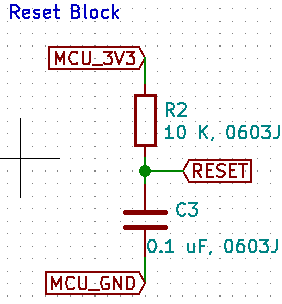
\includegraphics[scale=1]{reset_ckt.png}
	\end{figure}
	
	\textbf{Value Calculation}	
	\paragraph{R2}
	is acting as pull-up resistor here, which is used for high voltage programming (10V - 12V). Recommended value of pull-up resistor is 10 K$\Omega$.
	
	\paragraph{C3} 
	is used to filter high frequency noise, typical value is 100 nF (or 0.1 $\mu$F).
	
	\textbf{Power Calculation}
	
	Maximum allowable voltage for $V_{cc}$ is 5.5 V and $ V_{thresh}$ for reset pin detection is 1.1 V (cite datasheet here). 
	\begin{itemize}
		\item[R2:] consumes less than 0.1 w(equation \ref{eq:R2}), using 0603 \gls{smd} package.
				\\$P = \frac{V^{2}}{R} $\\
				$V = 5.5 V (max)$\\
				$R_{2} = 10 K\Omega $\\
				\begin{equation}
				P = 3.025 mW \label{eq:R2}
				\end{equation}	
		\item[C3:]	Max current flow through C3 is given by equation \ref{eq:C3}. Here I = 0.55 mA, Power = 3.025 mW, so using a 0603 \gls{smd} package, since 0603 provides with 0.1 W power rating.
			\begin{equation}
				I = \frac{V}{R_{2}}
				\label{eq:C3}
			\end{equation}	
			$ P = VI $	\\
			$ P = 3.025 mW \\ $
		\item[f:] The RC circuit also act as a \gls{lpf}, the cut-off frequency of RC filter is given by equation \ref{eq:f_reset}.
		
			\begin{equation}
				f = \frac{1}{2\pi RC}
				\label{eq:f_reset}
			\end{equation}	
			$ f = 159.15 $ Hz, so all high frequency noise is filtered out by this RC filter thus enhancing the performance of \gls{mcu} in noisy environment and preventing unwanted reset.				
	\end{itemize}
	
%http://www.ti.com/interface/circuit-protection/esd-protection-and-tvs-surge-diodes/support-training.html
% End - Hardware/Control Unit/Reset